\documentclass{article}
\usepackage[utf8]{inputenc}
\usepackage[letterpaper, portrait, margin=1in]{geometry}
\usepackage{multicol}
\usepackage{amsmath}
\usepackage{amssymb}
\usepackage{enumerate}
\setlength\parindent{0pt}
\usepackage{enumerate}
\usepackage{graphicx}
\graphicspath{ {./images/} }
\usepackage{fancyhdr}
\usepackage{tcolorbox}
\hyphenchar\font=-1
\usepackage{tabularx}

\newcommand{\header}[1]{\begin{large}\noindent #1\end{large}\\\rule{\textwidth}{0.5pt}}
\newcommand{\gap}{\medskip\\}
\newcommand{\centertext}[1]{\begin{center}#1\end{center}}
\newcommand{\bfrac}[2]{\left(\frac{#1}{#2}\right)}
\newcommand{\formula}[3]{\begin{center} \begin{tcolorbox}[title = #2] $$#3$$\end{tcolorbox}\end{center}}
\newcommand{\where}{\hspace{0.5cm} \textrm{where} \hspace{0.5cm}}
\newcommand{\hgap}{\hspace{0.5cm}}
\newcommand{\pfrac}[2]{\frac{\partial #1}{\partial #2}}
\newcommand{\sheader}[1]{\underline{#1:}}
\newcommand{\doubleformula}[4]{\begin{center} \begin{tcolorbox}[title = #2] $$#3$$\\$$#4$$\end{tcolorbox}\end{center}}
\newcommand{\curly}[1]{\left\{#1\right\}}
\newcommand{\proj}[2]{{}\textrm{proj}_{#1}\left(#2\right)}

\newcommand{\ds}{\displaystyle}
\newcommand{\Arg}{\textrm{Arg}}

\newcommand{\tripleformula}[5]{\begin{center} \begin{tcolorbox}[title = #2] $$#3$$\\$$#4$$\\$$#5$$\end{tcolorbox}\end{center}}

\usepackage{physics}
% \usepackage{braket}

\begin{document}
    \begin{center}
        \Large PHYS 304 Review Notes\\
        \normalsize Reese Critchlow
    \end{center}

    \header{General Forms for Solving Schrodinger Equations in Bound States}

    For a Schrodinger equation of the form:
    \begin{align*}
        -\frac{\hbar}{2m} \frac{\partial^2 \psi}{\partial x^2} + V(x) \psi = i\hbar \frac{\partial \psi}{\partial t},
    \end{align*}
    we can define a general solution for bound states to be of the 
    following form:
    \begin{align*}
        \Psi(x, t) = \sum_{n=0}^{\infty} c_n \psi_n(x) \cdot \varphi_n(t),
    \end{align*}
    where $\psi_n(x)$ is a \underline{stationery state} for the given potential
    $V(x)$, and $\varphi_n(t)$ is the time-dependance of the solution,
    given by:
    \begin{align*}
        \varphi_n(t) = e^{-iE_n t/\hbar},
    \end{align*}
    where $E_n$ is the energy corresponding to the state. In addition, 
    the bound state coefficients can be found according to:
    \begin{align*}
        c_n = \int_{-\infty}^\infty \psi_n(x) \Psi(x, 0)dx.
    \end{align*}
    These $c_n$ values can be interpreted as the probabilities of 
    each energy state:
    \begin{align*}
        P(E_n) = |c_n|^2
    \end{align*}
    and as a consequence:
    \begin{align*}
        \sum_{n = 1}^\infty |c_n|^2  = 1 && \textrm{and} && \langle H \rangle  = \sum_{n = 1}^\infty |c_n|^2 E_n. 
    \end{align*}
    \gap
    For the potentials that have been covered thus far in the course,
    there are two different stationery states corresponding to each 
    potential. We can also define their energies:

    \begin{multicols}{2}
        \centertext{\underline{Infinite Square Well}}
        \begin{align*}
            \psi_n &= \sqrt{\frac{2}{a}}\sin\left(\frac{n\pi}{a}x\right)\\
            E_n &= \frac{\hbar^2 k_n^2}{2m} = \frac{n^2 \pi^2 \hbar^2}{2ma^2}
        \end{align*}
        \centertext{where $k_n = \frac{n\pi}{a}$}
        \vfill\null
        \columnbreak
        \centertext{\underline{Harmonic Oscillator}}
        \begin{align*}
            \psi_n &= \left(\frac{m\omega}{\pi \hbar}\right)^{\frac{1}{4}} \frac{1}{\sqrt{2^n n!}}H_n(\xi)e^{-\xi^2/2}\\
            E_n &= \left(n + \frac{1}{2}\right) \hbar \omega
        \end{align*}
        \centertext{where $\ds \xi = \sqrt{\frac{m\omega}{\hbar}}x$}
        \vfill\null
    \end{multicols}

    The \underline{Hermite Polynomials} are also important to note:
    \begin{align*}
        H_n(\xi) = \begin{cases}
            H_0(\xi) = 1 \\
            H_1(\xi) = 2\xi\\
            H_2(\xi) = 4\xi^2-2\\
            H_3(\xi) = 8\xi^3 - 12\xi\\
            \ldots
            \end{cases}
    \end{align*}

    \pagebreak

    \sheader{Stationery States} Stationery states are states in which:
    \begin{enumerate}
        \item All expectation values are independent of time.
        \item Total energy is definite.
        \item The general solution is a linear combination of stationery
        states.
    \end{enumerate}

    \sheader{Key features of the stationery states of the infinite square well}
    \begin{itemize}
        \item They are alternating even and odd.
        \item Each successive energy state gains an additional zero 
        crossing (node)
        \item They are mutually orthogonal, which implies that $\ds \int \psi_m^*(x) \psi_n(x) = 0, m \neq n$.
    \end{itemize}

    It is also useful to know what the bound states look like for
    the harmonic oscillator.

    \begin{center}
        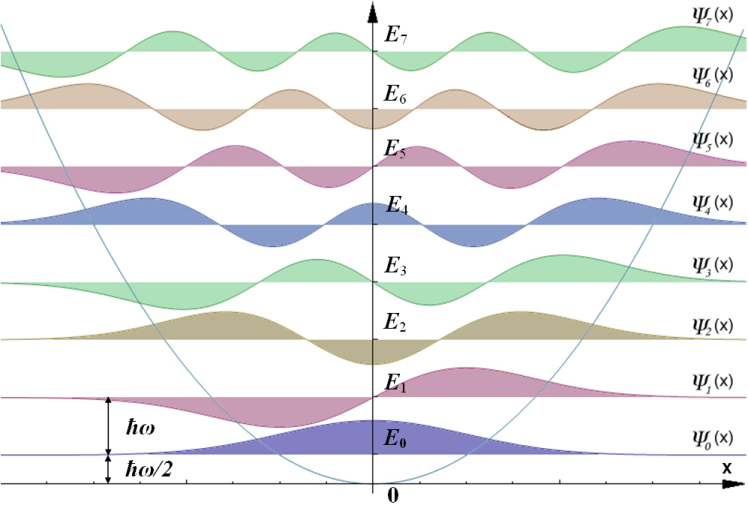
\includegraphics[scale=0.3]{harmonic-oscillator-states.png}
    \end{center}

    \header{General Forms for Solving Free Particle Problems}

    For many potentials, particles appear in \underline{scattered states},
    instead of bound states. In these cases, energies are not quantized
    and general forms are computed over integrals, not sums.
    \gap
    For the case of the \underline{free particle}, where the 
    potential is zero everywhere, one can find the solution using the
    following procedure.
    \begin{enumerate}
        \item Identify $\phi(k)$, which is the distribution of states 
        over the variable $k$, using a Fourier transform:
        \begin{align*}
            \phi(k) = \frac{1}{\sqrt{2\pi}} \int_{-\infty}^{\infty}\Psi(x, 0)e^{-ikx}dx.
        \end{align*}
        \item Transform the function out of the frequency domain using 
        another Fourier transform: 
        \begin{align*}
            \Psi(x,t) = \frac{1}{\sqrt{2\pi}}\int_{-\infty}^{\infty} \phi(k) e^{i\left(kx - \frac{\hbar k^2}{2m}t\right)} dk.
        \end{align*}
    \end{enumerate}

    The distribution of states $\phi(k)$ in the general solution is known 
    as the \underline{wavepacket}. There are two velocities that are important
    in this case.
    \begin{itemize}
        \item \sheader{Phase Velocity} $\ds v_\textrm{phase} = \frac{\omega}{k} = \frac{\hbar k}{2m} = \sqrt{\frac{E}{2m}}$
        \item \sheader{Group Velocity} $\ds v_\textrm{group} = 2v_\textrm{phase} = \frac{d\omega}{dk}$
    \end{itemize}
    In all of these forms, $k$ is $k_0$, which is the fundamental 
    frequency of the group.
    \gap

    \header{Probabilities and Expectation Values}
    \sheader{Heisenberg Uncertainty Principle}
    \begin{align*}
        \sigma_x \sigma_p \geq \frac{\hbar}{2}
    \end{align*}

    \header{Orthogonality}

    \begin{itemize}
        \item The stationery states in the infinite square well are orthogonal.
        \item $\ds \int_{0}^{L} \sin \left(\frac{n\pi x}{L}\right) \sin \left(\frac{m\pi x}{L}\right) dx = 0 $
        \item $\ds \int_{0}^{L} \cos \left(\frac{n \pi x}{L}\right) \cos \left(\frac{m \pi x}{L}\right) dx = 0$
        \item $\ds \int_{0}^{L} \sin \left(\frac{n \pi x}{L}\right) \cos \left(\frac{m \pi x}{L}\right) dx = 0$
        \item $\ds \int f_\textrm{even}(x) f_\textrm{odd}(x) dx = 0$
        \item $\ds \int_{0}^{L} \sin \left(\frac{n\pi x}{L}\right) \sin \left(\frac{n\pi x}{L}\right) dx = \frac{L}{2}$
        \item $\ds \int_{0}^{L} \cos \left(\frac{n\pi x}{L}\right) \cos \left(\frac{n\pi x}{L}\right) dx = \frac{L}{2}$
    \end{itemize}

    \header{Probabilites and Such}

    We can define the probability of an event $j$ given the total number of 
    events $N$ and the total number of times it occurs $N(j)$:
    \begin{align*}
        P(j) = \frac{N(j)}{N}.
    \end{align*}
    In discrete variables, if we seek to find the average event $j$, denoted by
    $\langle j \rangle$, we can find it with:
    \begin{align*}
        \langle j \rangle = \frac{\sum j N(j)}{N} = \sum_{j = 0}^\infty j P(j).
    \end{align*}

    The \underline{standard deviation} of an event is important to define:
    \begin{align*}
        \sigma = \sqrt{\langle j^2 \rangle - \langle j \rangle^2}
    \end{align*}

    Similar formulae can also be applied to continuous variables. First, we 
    define the \underline{probability density} of some quantity as $\rho(x) dx$,
    that is $\rho(x)dx$ is the probability that an individual (chosen at random)
    lies between $x$ and $(x + dx)$. Hence, it follows that:
    \begin{align*}
        P_{ab} = \int_a^b \rho(x) dx.
    \end{align*}

    \pagebreak 

    \header{Expected Values}

    As alluded to prior, we can have certain \underline{expected values} for quantities,
    that is, the average value for that quantity over all time. In general, for some quantity $Q$, this is given
    by:
    \begin{align*}
        \langle Q(x, p) \rangle = \int_{-\infty}^{\infty} \Psi^* \left[Q\left(x, -i\hbar \frac{\partial}{\partial x}\right)\right]\Psi dx
    \end{align*}
    Where $Q(x,p)$ is some operator that can be described as a function of $x$ and $p$.
    \gap
    Hence, we can define some common operators:
    \begin{itemize}
        \item \sheader{Position Operator, $x$} $x$.
        \item \sheader{Momentum Operator, $\hat{p}$} $\hat{p} = -i\hbar \frac{\partial}{\partial x}$.
    \end{itemize}
    Energy is another expected value, but obtaining it in bound states is a bit difficult.
    It can be obtained as follows:
    \begin{align*}
        \langle E \rangle = \sum_{n = 1}^\infty |c_n|^2 E_n.
    \end{align*}

    \header{Important Integrals}

    There are some important integrals that often come up:
    \begin{align*}
        \int_{-\infty}^\infty e^{-\frac{x^2}{a^2}}dx = \sqrt{\pi} a && \int_{-\infty}^\infty x^2 e^{-\frac{x^2}{a^2}} dx = \frac{\sqrt{\pi} a^3}{2}
    \end{align*}

    \pagebreak

    \header{Dirac Notation}

    \sheader{Definitions}
    \begin{itemize}
        \item A \underline{ket}, denoted as $\ket{B}$ defines notation for a vector. Hence, it 
        can be interpreted that:
        \begin{align*}
            \ket{B} &= \begin{bmatrix}
                b_1 \\
                b_2 \\
                \vdots \\
                b_n
            \end{bmatrix}
        \end{align*}
        \item A \underline{bra}, denoted as $\bra{A}$ defines notation for the complex conjugate 
        of a vector. Hence, it can be interpreted that:
        \begin{align*}
            \bra{A} &= \begin{bmatrix}
                a_1 \\
                a_2 \\
                \vdots \\
                a_n
            \end{bmatrix}^\dagger = 
            \begin{bmatrix}
                a_1^* & a_2^* & \cdots & a_n^*
            \end{bmatrix}
        \end{align*}
    \end{itemize}
    \sheader{Mathematical Implications}
    \begin{itemize}
        \item Thus, it follows that the combination of a bra and ket in order yields the inner product 
        of two vectors:
        \begin{align*}
            \braket{A}{B} = \begin{bmatrix} a_1^* & a_2^* & \cdots & a_n^* \end{bmatrix} \begin{bmatrix}
                b_1 \\
                b_2 \\
                \vdots \\
                b_n
            \end{bmatrix} = a_1^* b_1 + a_2^* b_2 + \cdots + a_n^* b_n
        \end{align*}
        \item We can also define the ``ketbra'' operation, which is the reverse order of the braket,
        and is also the \underline{outer product}. This is especially useful in the case of finding 
        the \underline{identity matrix} for a system:
        \begin{align*}
            \sum_{i} = \ketbra{e_i}{e_i} = I
        \end{align*}
        Where $e_i$ denote all of the possible basis vectors for a system.


    \end{itemize}

    \sheader{Applications in Quantum Physics}
    \gap
    In quantum mechanics, we introduce the concept of \underline{Hilbert Space}, which 
    under the viewpoint that a function can be described as an \underline{abstract vector},
    is defined as the vector space of all square-integrable functions on specified intervals:
    \begin{align*}
        \curly{f(x) : \int_a^b |f(x)|^2 dx < \infty}
    \end{align*}
    Since most functions are map continuous functions to continuous functions in quantum 
    physics, we can use braket notation and Hilbert Space to express the inner product 
    for two functions:
    \begin{align*}
        \braket{f(x)}{g(x)} = \int_a^b f(x)^* g(x)dx
    \end{align*}
    where $a$ and $b$ denote endpoints of the $f(x)$ and $g(x)$ abstract vectors. Oftentimes,
    these bounds are infinite. A corollary of this is that if both $f$ and $g$ are square integrable
    functions, then the inner product between $f$ and $g$ $\braket{f}{g}$ is guaranteed to exist.
    \pagebreak
    \gap
    There are some important implications that arise from these definitions:
    \begin{itemize}
        \item A function is said to be \underline{normalized} when its inner product with itself 
        evaluates to 1.
        \item Two functions are \underline{orthogonal} to each other when their inner product 
        is zero.
        \item Two functions are \underline{orthonormal} if their inner product is zero and they 
        are normalized.
        \item A set of functions is \underline{complete} if \textbf{any} other function $f$ in 
        Hilbert Space can be expressed as a linear combination of the two:
        \begin{align*}
            f = \sum_{n=1}^\infty c_n f_n(x)
        \end{align*}
        where for an orthonormal set, $c_n = \braket{f_n}{f}$.
        \begin{itemize}
            \item Infinite Square Well states are complete on $(0, a)$.
            \item Harmonic Oscillator states are complete on $(-\infty, \infty)$.
        \end{itemize}
    \end{itemize}

    \sheader{Observables}
    If we state that wavefunctions can be represented as abstract vectors, then 
    we can state that observables correspond to linear transformations on wavefunctions.
    Hence, to compute an observable, we can imagine the process as:
    \begin{enumerate}
        \item Transform the original wavefunction $\Psi$ using some linear transformation
        representing the observable: $Q\ket{\Psi}$
        \item Project the original wavefunction onto the transformed space to obtain 
        the magnitude of the observable: $\bra{\Psi} Q \ket{\Psi}$
    \end{enumerate}
    Hence, we can state that for some observable $Q$: 
    \begin{align*}
        \langle Q \rangle = \expval{Q}{\Psi} = \int_{-\infty}^\infty \Psi^* \hat{Q} \Psi dx
    \end{align*}
    It is important to note that since we require observables to be real quantities, 
    that all operators for an observable must be \underline{hermetian}, that is that 
    $\hat{Q} = \hat{Q}^\dagger$, or for the purpose of proofs:
    \begin{align*}
        \braket{f}{\hat{Q} f} = \braket{\hat{Q} f}{f}
    \end{align*}
    \sheader{Determinate States and Eigenfunctions}
    \gap 
    It is known that \underline{determinate states of $Q$ are eigenfunctions of $\hat{Q}$}, that is:
    \begin{align*}
        \hat{Q}\psi = q \psi
    \end{align*}
    where $q = \langle Q \rangle$.
    From this, we obtain two important definitions:
    \begin{itemize}
        \item \sheader{Spectrum} the collection of all of the eigenvalues for a given wavefunction.
        \item \sheader{Degenerate Spectrums} spectrums where two or more linearly independent 
        eigenfunctions share the same eigenvalue.  
    \end{itemize}
    It is to be noted that there exists two types of spectra:
    \begin{itemize}
        \item \sheader{Discrete Spectra} Eigenvalues are separated from each other
        \begin{itemize}
            \item Eigenfunctions lie in Hilbert space (normalizable) and constitute physically 
            realizable states.
            \item Eigenvalues are real.
            \item Eigenfunctions are orthonormal to each other.
        \end{itemize}
        \item \sheader{Continuous Spectra} Eigenfunctions are non-countable, continuous, and 
        are not normalizable. As a result, they do not represent possible wavefunctions, however,
        a linear combination of them \textit{might} be.
        \begin{itemize}
            \item Eigenfunctions with real eigenvalues are said to be \underline{Dirac Normalizable} (notes on this later) 
            and complete.
        \end{itemize}
    \end{itemize}
    \sheader{Axiom ($\star$)} The eigenfunctions of an observable operator are \underline{complete}.

    \pagebreak

    \header{Generalized Statistical Interpretation}

    \sheader{Core Concepts}
    \begin{enumerate}
        \item  If you measure a measure an observable $Q(x, p)$ on a particle in the 
        state $\Psi(x, t)$, you are certain to get one of the eigenvalues of the 
        Hermetian operator $\hat{Q}$ ($\star \star$).
        \begin{enumerate}
            \item If the spectrum is \underline{discrete}, then the probability of getting 
            the particular eigenvalue $q_n$ associated with an orthonormal eigenfunction $f_n(x)$ is:
            \begin{align*}
                |c_n|^2 && \textrm{where} && c_n = \braket{f_n}{\Psi}, n \in \mathbb{N}
            \end{align*}
            \item If the spectrum is \underline{continuous}, with \textit{real} eigenvalues 
            $q(z)$ and associated [Dirac-Normalized] eigenfunctions $f_z(x)$, the probability of 
            getting a result in the range $dz$ is:
            \begin{align*}
                |c(z)|^2 dz && \textrm{where} && c(z) = \braket{f_z}{\Psi}, z \in \mathbb{R}
            \end{align*}
        \end{enumerate}
        \item By means of $(\star)$ and $(\star\star)$, it is implied that $\Psi$ is a linear 
        combination of functions for some basis:
        \begin{align*}
            \Psi = \sum_n c_n(t) f_n && \textrm{or} && \Psi = \int_{-\infty}^\infty c(z,t) f_z dz 
        \end{align*}
        \begin{enumerate}
            \item Combined with the fact that $\sum_n |c_n|^2 = 1$, it is also implied that we can describe expectation values in terms of 
            generalized probabilities:
            \begin{align*}
                \langle Q \rangle = \sum_n q_n |c_n|^2
            \end{align*}
        \end{enumerate}
    \end{enumerate}

    Given this, we can hypothesize what various different basis functions might 
    look like for different observables. Some examples (in position space) include:
    \begin{itemize}
        \item Momentum-Space Eigenfunctions: $f_p(x) = \frac{1}{\sqrt{2\pi \hbar}} e^\frac{ipx}{\hbar}$
        \item Position-Space Eigenfunctions: $g_y(x) = \delta(x-y)$
    \end{itemize}
    The existence of a momentum-space eigenfunction in position space provides us 
    with the ability to find the \underline{momentum space wavefunction}. It is 
    denoted as:
    \begin{align*}
        \Phi(p, t) = \frac{1}{\sqrt{2\pi \hbar}} \int_{-\infty}^\infty e^{\frac{-ipx}{\hbar}}\Psi(x,t)dx
    \end{align*}
    Which, if we look closer at, is actually a bra-ket in disguise:
    \begin{align*}
        \Phi(p, t) = \frac{1}{\sqrt{2\pi \hbar}} \int_{-\infty}^\infty e^{\frac{-ipx}{\hbar}}\Psi(x,t)dx
        = \braket{f_p(x)}{\Psi(x,t)}
    \end{align*}
    This serves as a nice segue into the next concept, which are \underline{bases in Hilbert space}.
    \gap
    \sheader{Bases in Hilbert Space} Since the Hilbert space is a space of functions which 
    can be expressed as abstract vectors, then there must be an arbitrary abstract vector in 
    Hilbert space corresponding to every possible wavefunction. This is denoted by 
    $\ket{\mathcal{S}(t)}$.
    \gap
    Before we move deeper, it is important to define some vectors that will be used 
    frequently in the following text:
    \begin{itemize}
        \item $\ket{x}$: eigenfunction of $\hat{x}$ with arbitrary eigenvalue $x$...*
        \item $\ket{p}$: eigenfunction of $\hat{p}$ with arbitrary eigenvalue $p$...*
        \item $\ket{n}$: eigenfunction ($E_n$ [constant]) of $\hat{H}$ with arbitrary eigenvalue $E$...*
    \end{itemize}
    *... I wrote ellipses in my notes and think I'm missing something here.

    \pagebreak

    Which leads to the important property that the inner product/projection of one 
    bases eigenfunctions with the arbitrary $\mathcal{S}(t)$ function yields the 
    wavefunction in that respective basis:
    \begin{itemize}
        \item $\braket{x}{\mathcal{S}(t)} = \Psi(x,t)$
        \item $\braket{p}{\mathcal{S}(t)} = \Phi(p,t)$
        \item $\braket{n}{\mathcal{S}(t)} = c_n(t)$
    \end{itemize}

    Hence, it is also to be noted that different operators ``look different'' in 
    different bases:
    \begin{align*}
        \hat{x} \to \begin{cases}
            x & \textrm{ in position space}\\
            i\hbar \frac{\partial}{\partial p} & \textrm{ in momentum space}
        \end{cases} &&
        \hat{p} \to \begin{cases}
            -i\hbar \frac{\partial}{\partial x} & \textrm{ in position space}\\
            p & \textrm{ in momentum space}
        \end{cases}
    \end{align*}

    \sheader{Remark} We can determine the coefficients for a function in its basis by:
    \begin{align*}
        \braket{f'_n}{f_n}
    \end{align*}
    for some arbitrary eigenfunction $f_n$ for some observable $\hat{Q}$.
    \gap
    Moving backwards, we can also find $\ket{\mathcal{S}(t)}$ for various bases:
    \begin{itemize}
        \item $\braket{\Psi(p,t)^*}{p} = \int \Psi(p,t) \ket{p}dp$
        \item $\braket{\Phi(x,t)^*}{x} = \int \Phi(x,t) \ket{x}dx$
    \end{itemize}
    However, since $\Phi(p, t) = \braket{p}{\mathcal{S}(t)}$ and $\Psi(x,t) = \braket{x}{\mathcal{S}(t)}$,
    we can generalize:
    \begin{align*}
        \ket{\mathcal{S}(t)} = \int_{-\infty}^\infty \expval{\mathcal{S}(t)}{O_z} dz
    \end{align*}
    for some arbitrary basis $\curly{\ket{O_z}}$.
    \gap
    \sheader{Change of Bases in Dirac Notation}
    Given everything that we know, it should make sense that we can measure observables 
    in different bases. To generalize, we can write that:
    \begin{align*}
        \bra{\textrm{basis}}\textrm{operator} \ket{\textrm{state}}
    \end{align*}
    Examples:
    \begin{itemize}
        \item $\bra{x}\hat{x}\ket{\mathcal{S}(t)} = x \Psi(x, t)$: application of position operator in $x$ basis.
        \item $\bra{p}\hat{x}\ket{\mathcal{S}(t)} = i\hbar\frac{\partial \Phi}{\partial p}$: application of position operator in $p$ basis.
    \end{itemize}

    \sheader{Notes on the concept of Dirac Orthonormality} In the case that eigenvalues are 
    discrete, the condition holds that:
    \begin{align*}
        \braket{f_n}{f_m} = \delta_{nm} = \begin{cases}
            0 & \textrm{if  } n \neq m\\
            1 & \textrm{if  } n = m
        \end{cases}
    \end{align*}
    However, since continuous states don't obey this kind of orthonormality with the Kronecker-Delta 
    function, they still are able to find a sort of orthonormality with the Dirac-Delta function:
    \begin{align*}
        \braket{f_q'}{f_q} = \delta(q - q')
    \end{align*}
    This makes sense, since the physical solution for systems with discrete eigenvalues is obtained under discrete summation,
    the Kronecker-Delta function fits the use case. Similarly, since the physical solution for 
    systems with continuous eigenvalues is obtained by integration, the Dirac-Delta function fits the use case.

    \pagebreak

    \header{Midterm Prep}

    In bra/ket notation, we generally see 5 main different types of ``things'':
    \begin{itemize}
        \item \sheader{States Associated with Bases} $\Psi(x,t)$, $\Phi(p, t)$, $n$
        \item \sheader{Arbitrary State} $\mathcal{S}(t)$
        \item \sheader{Eigenfunction Sets} $x, p, E_n, f_x, f_p$
        \item \sheader{Operators} $\hat{x}, \hat{p}, \hat{H}$
        \item \sheader{Stationery States} $\psi_n$
    \end{itemize}
    
\end{document}